\chapter{Online decision-making: competitive analysis and regret}

Online decision theory enters this corpus through systems doors: when to adapt a filter to a recurring false positive, whether to trust an ML oracle's prediction, how to clean a time series that has not yet arrived, how to tune a discretization knob. Four papers carry it---two via \emph{competitive analysis} \cite{sigmod26-242,sigmod26-094}, two via \emph{regret} \cite{sigmod26-140,sigmod26-221}, none an online-algorithms paper per se. They share one shape: the system commits to decisions while the input's future is unknown, and the committed sequence is judged against a hindsight optimum that sees everything. Two classical yardsticks quantify that gap, and choosing between them is this chapter's lesson.

\section{The tools}

\begin{definition}[Competitive ratio]
An online algorithm $A$ for a cost-minimization problem is \emph{$c$-competitive} if there is a constant $b$ such that
\[
\operatorname{cost}_A(\sigma) \;\le\; c\cdot\operatorname{cost}_{\mathrm{OPT}}(\sigma) + b
\qquad\text{for every input sequence }\sigma,
\]
where $\mathrm{OPT}$ is the offline optimum that observes all of $\sigma$---including where it ends---before acting.
\end{definition}

The canonical micro-example is \emph{ski rental}: skis rent for $1$ per day and cost $B$ to buy; each morning the skier learns only whether the season continues. Renting for $B$ days and then buying is $2$-competitive, and no deterministic algorithm does better; randomization lowers the barrier to $e/(e-1)\approx 1.58$ against an oblivious adversary~\cite{online-decisions-bg2}. The framework descends from the amortized analysis of list update and paging~\cite{online-decisions-bg1}. Figure~\ref{fig:ski-rental} shows the geometry; the memoryless ``when do I commit?'' structure is why this toy model reappears below in database clothing.

\begin{figure}[ht]
\centering
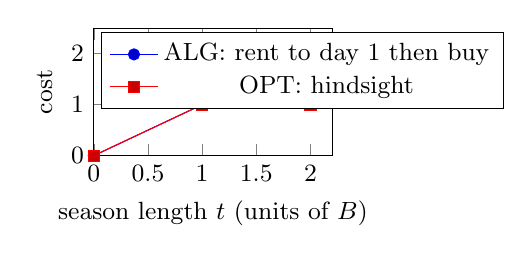
\begin{tikzpicture}
\begin{axis}[width=0.38\textwidth,height=3.2cm,
  xlabel={season length $t$ (units of $B$)}, ylabel={cost},
  xmin=0,xmax=2.2,ymin=0,ymax=2.5,
  legend pos=north west,legend style={font=\small},
  tick label style={font=\small},label style={font=\small}]
\addplot coordinates {(0,0) (1,1) (2,2)};
\addplot coordinates {(0,0) (1,1) (2,1)};
\legend{ALG: rent to day $1$ then buy,OPT: hindsight}
\end{axis}
\end{tikzpicture}
\caption{Ski rental with rent $1$ and buy price $B=1$: rent-to-$B$-then-buy matches OPT while $t<B$ and never exceeds $2\cdot\mathrm{OPT}$.}
\label{fig:ski-rental}
\end{figure}

\begin{definition}[Regret]
For decisions $a_1,\dots,a_T$, where round $t$ charges a loss $\ell_t(a_t)$ revealed only after the decision, the \emph{regret} against the best fixed comparator is
\[
R_T \;=\; \sum_{t=1}^{T}\ell_t(a_t)\;-\;\min_{a\in\mathcal{A}}\sum_{t=1}^{T}\ell_t(a).
\]
An algorithm is \emph{no-regret} if $R_T=o(T)$: its average loss converges to that of the best action chosen once, in hindsight.
\end{definition}

In the stochastic multi-armed bandit ($K$ actions, rewards in $[0,1]$ with fixed unknown means, only the chosen arm's reward observed), UCB plays the arm with the highest optimism index $\bar r_k+\sqrt{2\ln t/n_k}$ and achieves $R_T=O(\sqrt{KT\log T})$~\cite{online-decisions-bg3}; adversarial and unified views are surveyed in~\cite{online-decisions-bg4}. In short: the \emph{competitive ratio} prices the unknown future---unrestricted adversary, switching comparator, guarantee on every input---for one-shot commitments under adversarial workloads; \emph{regret} prices ignorance of a distribution---repeated rounds, per-round feedback, fixed comparator, $O(\sqrt{T})$ bound---for stochastic tuning loops.

\section{Four exemplars from the corpus}

\subsection{Ski rental inside a sketch filter}

A streaming distinct-count filter occasionally yields a false positive; each repeat costs a database lookup $C_{DB}$, adapting the entry costs an extra reverse-map lookup $C_{RM}=\alpha\,C_{DB}$, and after adapting both costs stop. Whether and when to adapt is ski rental in disguise---rental price $C_{DB}$, purchase price $C_{DB}+C_{RM}$, adversarial arrival stream.

\begin{theorem}[Adapt after $\lfloor\alpha\rfloor$ repeats; 2-competitive]
If $\alpha\ge 1$, i.e., the cost of querying the reverse map is greater than a database lookup, the optimal deterministic strategy is to adapt immediately after the false positive repeats $\lfloor\alpha\rfloor$ times, and is 2-competitive.
\end{theorem}

\begin{remark}[The golden-ratio threshold]
For $\alpha<1$ the two candidate policies have ratios $1+\alpha$ (adapt immediately) and $(2+\alpha)/(1+\alpha)$ (adapt on the second false positive); these cross where $\alpha^2+\alpha-1=0$, i.e.\ at $\alpha=(\sqrt{5}-1)/2\approx 0.618$. The optimal rule: adapt immediately when $\alpha<0.618$, adapt on the second occurrence otherwise.
\end{remark}

The competitive ratio is the right yardstick: the arrival stream is adversarial and the offline comparator knows when the repeats end. The skeleton also composes---augmenting a strongly adaptive filter with this routine bounds false positives by $(1+\lceil\alpha\rceil)\bigl(n\epsilon+O(\sqrt{n\epsilon\log n+\log n})\bigr)$ with high probability, the 2-competitive core living inside a high-probability bound. \cite{sigmod26-242}

\subsection{Paying for oracle predictions at enumeration time}

Subgraph-isomorphism (\textsc{SubIso}) enumeration is accelerated by an ML oracle that prunes the search at prediction cost $f(Q,M)$, but a wrong prediction misses matches. The paper's $\beta$-robustness---extra output cost relative to the optimal exact enumerator---is a competitive ratio; the general case is barred, then per-algorithm ratios are proved.

\begin{theorem}[No constant robustness in general]
No algorithm exists for \textsc{SubIso} that is both output polynomial and $\beta$-robust for any positive constant $\beta$ unless $\mathrm{fewP}=P$, where $\mathrm{fewP}$ denotes the class of problems recognizable by a nondeterministic Turing machine in polynomial time with only polynomially many solutions.
\end{theorem}

For the paper's oracle-guided hybrids the matching upper bounds are constant competitive ratios, e.g.\ $5N_c\,(f(Q,M)+2|G|\,|Q|)$ for $\mathrm{VF3}_M$ with probability at least $1-\epsilon$, proved via a generalized Bonferroni inequality over the oracle's false predictions. The barrier is a parsimonious reduction; the ratios fit competitive analysis since the graph is arbitrary and the comparator is the exact enumerator's cost---paid in oracle calls and output quality rather than money. \cite{sigmod26-094}

\subsection{Windowed time-series repair with decay regret}

Given a multivariate time series violating soft and hard constraints, the offline optimal repair is computed exactly as the maximum-weight path in a DAG over anchor points. The online algorithm is the same dynamic program restricted to a sliding window of width $W$, so its regret is precisely what the truncated lookback misses.

\begin{theorem}[Exponentially decaying window regret]
The regret $R_n$ of the online algorithm is bounded:
\[
R_n \;=\; \sum_{i=1}^{n} r_i \;\le\; \sum_{i=1}^{n} e^{-\beta(W+1)} \;=\; n\,e^{-\beta(W+1)},
\]
where each one-step regret $r_i$ compares the score of the offline optimal anchor point with that of the best anchor visible within the window, and the strictly decreasing path weights obey $\gamma(\Delta)\le e^{-\beta\Delta}$.
\end{theorem}

The comparator is a best \emph{sequence} (the exact offline optimum), a competitive-analysis comparator, yet the guarantee is a sum of per-step gaps in the regret style; the exponential decay makes a bounded window affordable---each extra unit of window multiplies the neglected tail by $e^{-\beta}$. \cite{sigmod26-221}

\subsection{Attribute discretization as a bandit}

Choosing how to bin numerical attributes is posed as maximizing $J(B,D)=\alpha\,M_{\mathrm{sem}}(B)+(1-\alpha)\,M_{\mathrm{util}}(B,D)$ over partition sets, with the search organized as an MDP over clusters of similar partitions. The only provable guarantee comes from the case where the search collapses to a repeated choice among $K$ cluster-arms.

\begin{theorem}[The single-attribute case is exactly a $K$-armed bandit]
If (i) $d=1$ (single attribute, one action per episode) and (ii) MCC uses the UCB index for action selection and updates, then Algorithm 1 becomes a UCB-guided MCC variant and reduces exactly to a stochastic multi-armed bandit with $K$ arms (one per cluster) and reward in $[0,1]$ given by $J$; this equivalence does not extend to the multi-attribute case ($d>1$). Running Algorithm 1 for $T$ episodes yields the regret guarantees inherited from UCB: gap-free regret $O(\sqrt{KT\log T})$.
\end{theorem}

This is the reduction school of regret usage: engineer the system so an existing bandit theorem applies verbatim and inherit $O(\sqrt{KT\log T})$ for free. Regret fits because episodes repeat with stochastic rewards in $[0,1]$ and the comparator is the best fixed cluster; for $d>1$ the equivalence breaks and no guarantee is claimed. \cite{sigmod26-140}

\begin{reachbox}{When to reach for competitive analysis vs regret}
\begin{itemize}
\item \textbf{Competitive ratio}: the decision is a commitment (adapt, buy, rebuild, trust an oracle) under a possibly adversarial input, and you need a guarantee on \emph{every} run---ski-rental-shaped trade-offs between a repeated small cost and a one-time large one. Deterministic bounds are typically $2$; randomization usually improves them once an adversary model is fixed.
\item \textbf{Regret}: the same decision repeats over many rounds with per-round feedback and tacit stochasticity---tuning, configuration search, repair over stationary error processes. The comparator is a \emph{fixed} action in hindsight; the $O(\sqrt{T})$ bound is weak per run, strong on average.
\item \textbf{Hybrids are the corpus pattern}: reduce the system to a $K$-armed bandit and inherit UCB's bound wholesale; wrap a 2-competitive sub-routine inside a high-probability filter bound; measure a windowed online heuristic against the exact offline DP with a decay argument.
\item \textbf{Check before you cite}: regret needs normalized rewards (here $[0,1]$) and a defined feedback model; a competitive ratio needs a well-defined offline optimum and, if randomized, an oblivious adversary.
\end{itemize}
\end{reachbox}
